\section{Kiến trúc hệ thống}

\subsection{Tổng quan}

Hệ thống gồm ba dịch vụ chạy trong Docker Compose và một giao diện web tĩnh. Chỉ dịch vụ ứng
dụng mở cổng ra máy chủ; hai dịch vụ còn lại nằm trong mạng nội bộ của compose nên không va
chạm với các stack khác trên cùng máy.

\begin{figure}[htbp]
\centering
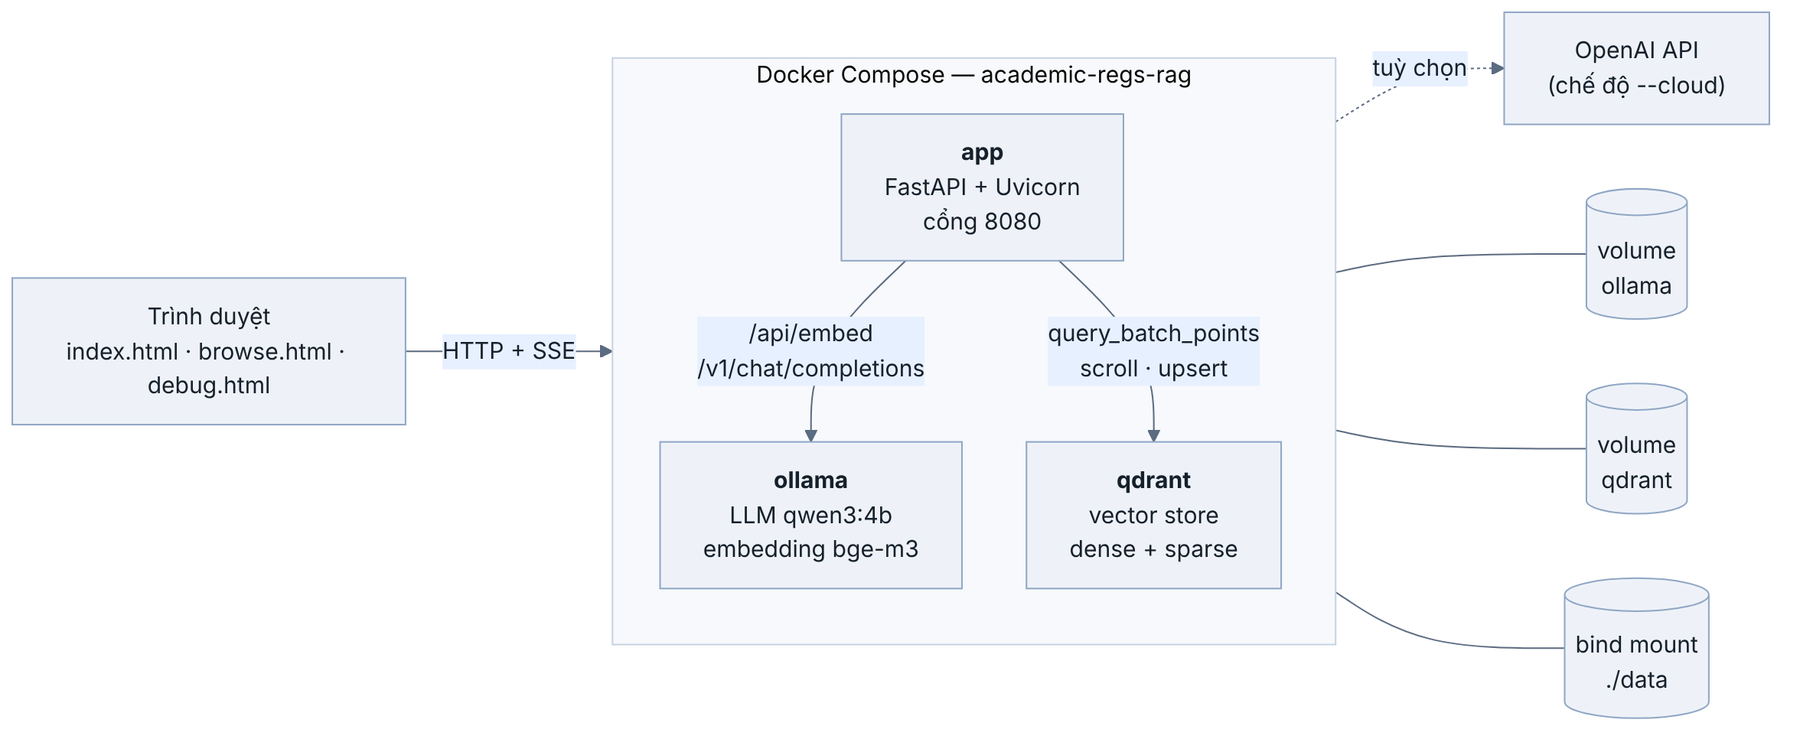
\includegraphics[width=\textwidth]{img/kien-truc.png}
\caption{Kiến trúc triển khai. Toàn bộ mô hình chạy tại chỗ; đường nét đứt tới OpenAI chỉ được
dùng khi khởi động ở chế độ \code{--cloud}, và kể cả khi đó thì embedding vẫn chạy local nên
không phải nạp lại dữ liệu.}
\label{fig:kientruc}
\end{figure}

\subsection{Các thành phần}

\begin{rtable}
\begin{tabular}{@{}p{0.17\textwidth} p{0.26\textwidth} p{0.47\textwidth}@{}}
\toprule
\tabhead{\textbf{Thành phần}} & \tabhead{\textbf{Công nghệ}} & \tabhead{\textbf{Vai trò}} \\
\midrule
\textbf{app} & FastAPI + Uvicorn, Python 3.11 &
  API HTTP, luồng SSE, pipeline truy xuất, phục vụ ba trang giao diện \\
\textbf{ollama} & Ollama, \code{qwen3:4b}, \code{bge-m3} &
  Sinh câu trả lời và tạo vector embedding, chạy hoàn toàn local \\
\textbf{qdrant} & Qdrant v1.15 &
  Lưu 90 điểm vector, mỗi điểm có một vector dense và một vector sparse \\
\textbf{Giao diện} & HTML + CSS + JavaScript thuần &
  Ba trang: hỏi đáp, tra cứu, chẩn đoán. Không framework, không CDN \\
\textbf{Dữ liệu} & bind mount \code{./data} &
  PDF gốc, Markdown đã rà soát, manifest nạp dữ liệu, log truy vấn \\
\bottomrule
\end{tabular}
\captionof{table}{Thành phần hệ thống và vai trò.}
\label{tab:thanhphan}
\end{rtable}

\subsection{Cơ sở lựa chọn công nghệ}

\begin{itemize}
  \item \textbf{Ollama thay vì gọi API đám mây.} Ràng buộc “chạy tại chỗ” là ràng buộc cứng.
  Ollama cung cấp sẵn giao diện tương thích OpenAI \cite{ollama}
  (\code{/v1/chat/completions}), nên cùng một đoạn mã khách hàng dùng được cho cả Ollama,
  OpenAI và vLLM — đổi nhà cung cấp chỉ là đổi biến môi trường.
  \item \textbf{Qdrant thay vì FAISS hay pgvector.} Qdrant hỗ trợ vector thưa có sẵn cơ chế IDF
  phía máy chủ, lọc theo trường payload, và gửi nhiều truy vấn trong một request
  (\code{query\_batch\_points}) \cite{qdrant} — ba tính năng mà pipeline này dùng trực tiếp.
  \item \textbf{bge-m3.} Đa ngôn ngữ, chất lượng tiếng Việt tốt, 1024 chiều, chạy được CPU.
  Quan trọng hơn: embedding luôn chạy local kể cả ở chế độ cloud, nên việc đổi mô hình sinh
  không bao giờ buộc phải nạp lại toàn bộ dữ liệu.
  \item \textbf{qwen3:4b.} Đủ nhỏ để chạy trên laptop, tiếng Việt chấp nhận được. Chế độ suy
  luận (“thinking”) được tắt bằng chỉ thị \code{/no\_think} vì nó làm chậm đáng kể mà không cải
  thiện chất lượng cho tác vụ tóm lược có nguồn.
  \item \textbf{Giao diện không framework.} Toàn bộ giao diện là ba file HTML và một file CSS,
  không phụ thuộc CDN. Hệ quả: hệ thống chạy được trong mạng hoàn toàn cô lập, và không có bước
  build nào giữa mã nguồn và sản phẩm.
\end{itemize}

\chapterbreak
